\chapter{OpenBTS}

OpenBTS is a Unix application that uses a software radio to present a GSM Um interface 
to handsets and uses a SIP softswitch or PBX to connect calls.
The combination of the global-standard GSM air interface with low cost VoIP backhaul 
forms the basis of a new type of cellular network that can be deployed and operated at a much lower
cost than existing technologies in many applications, 
especially rural cellular deployments and private cellular networks in remote areas.

\section{The OpenBTS Application Suite}
A complete OpenBTS installation consists of many distinct applications:

\begin{itemize}
\item \textbf{OpenBTS --} The actual OpenBTS application, containing most of
the GSM stack above the radio modem.
\item \textbf{Transceiver --} The software radio modem and hardware control interface.
\item \textbf{SMQueue --} A store-and-forward server for text messaging.
\item \textbf{Asterisk --} A VoIP PBX or ``softswitch''.
\item \textbf{SIPAuthServe --} An application managing the database of subscriber information.
\item \textbf{Other Services --} Optional services supported through 
external servers, interfaced to OpenBTS through various protocols.
\end{itemize}

\section{Key applications}
\subsection{OpenBTS}
The OpenBTS application contains:
\begin{itemize}
\item L1 TDM functions
\item L1 FEC functions
\item L1 closed loop power and timing controls
\item L2 LAPDm
\item L3 radio resource management functions
\item L3 GSM-SIP gateway for mobility management
\item L3 GSM-SIP gateway for call control
\item L4 GSM-SIP gateway for text messaging
\end{itemize}

The general design approach of OpenBTS is not to implement any function above L3 or L4, so at L3 or L4
every subprotocol of GSM is either terminated locally or translated through a gateway to some other protocol
for handling by an external application. Similarly, OpenBTS itself does not contain any speech transcoding
functions above the L1 FEC parts.


\subsection{Transceiver}
The transceiver application performs the radiomodem functions of GSM 05.05 and manages 
the Gigabit Ethernet interface
(USB2 interface, in case
of USRP1 or older models) to the radio hardware.

\subsection{SMQueue}
SMQueue is a store-and-forward server that is used for 
text messaging in the OpenBTS system. SMQueue is required to send 
a text message from one MS to another, or to an MS from any source.

\subsection{SIP router/PBX}

OpenBTS uses a SIP router or PBX to perform the 
call control functions that are normally performed by the MSC
in a conventional GSM network. These switches also provide transcoding 
services.

The SIP router used in OpenBTS is Asterisk by default. Though there are other
PBXs available in the market like Yate, FreeSwitch, etc.

\subsection{SIPAuthServe}
An application that implements Subscriber Registry, the database of subscriber 
information that replaces both the Asterisk SIP registry and the GSM Home 
Location Register (HLR) found in a conventional GSM network.

\section{Network organization}
In the simplest network, with just a single access point, all the applications run
on the same embedded computer as shown in figure~\ref{fig:btsSimple}.

In larger network, with more than one access points, one of them can behave as a master and provide servers to the rest of them.
Figure~\ref{fig:btsLarge} shows a network with two access points where
a master access points is providing servers to the other one.

The Transceiver applications and the OpenBTS must run in each GSM/SIP access point. 
The Asterisk and the Subscriber Registry applications (SIPAuthServe) 
communicate via the filesystem, so they must run in the same computer,
but that computer can be remote to the access point. 
SMQueue and other servers can run in any access point and can have 
multiple instances.
\begin{figure}
  \centering
    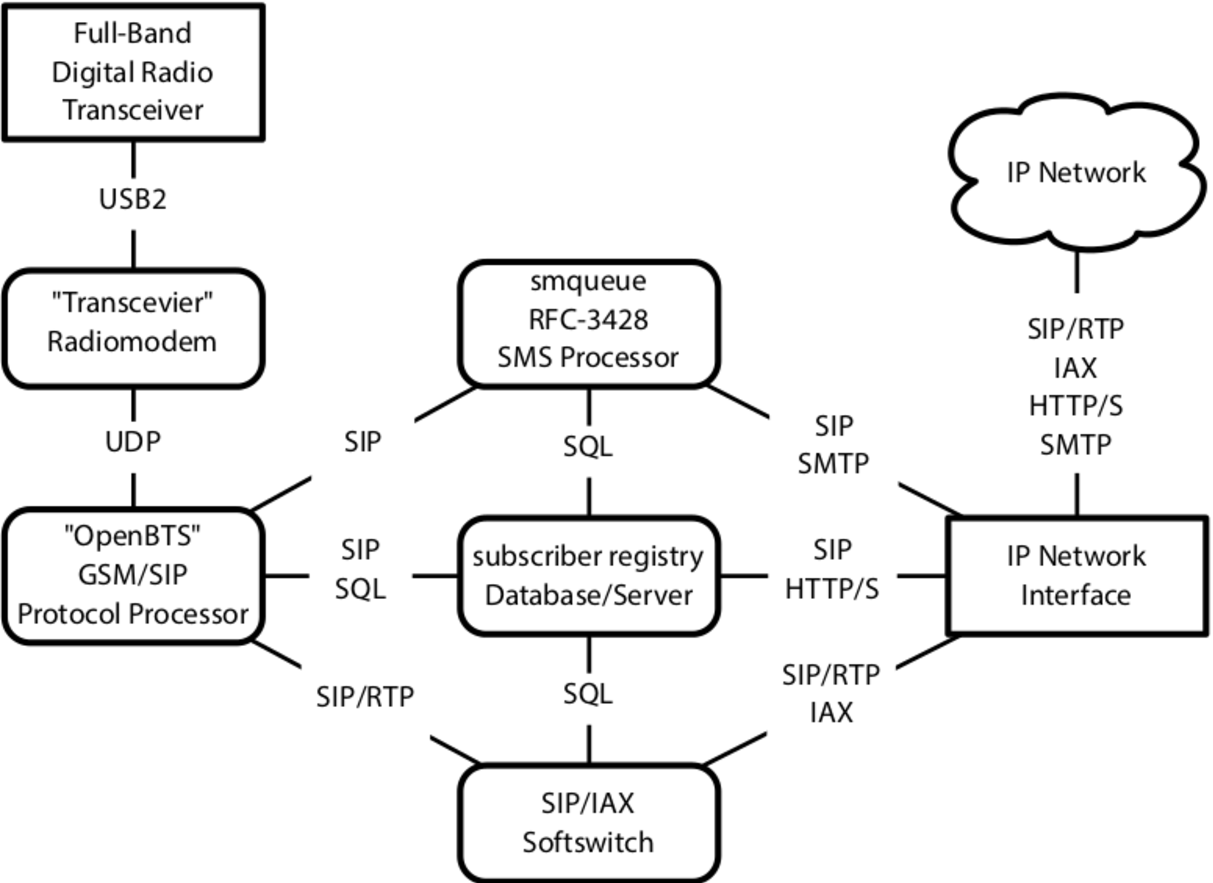
\includegraphics[width=\textwidth]{btsSimple}
  \caption[Simplest OpenBTS network]{Components of the OpenBTS application suite 
  and their communication channels as installed in each
access point. Sharp-cornered boxes are hardware components.
Round-cornered boxes are software components \protect\cite{openbtsMan}.}
  \label{fig:btsSimple}
\end{figure}

\begin{figure}
  \centering
    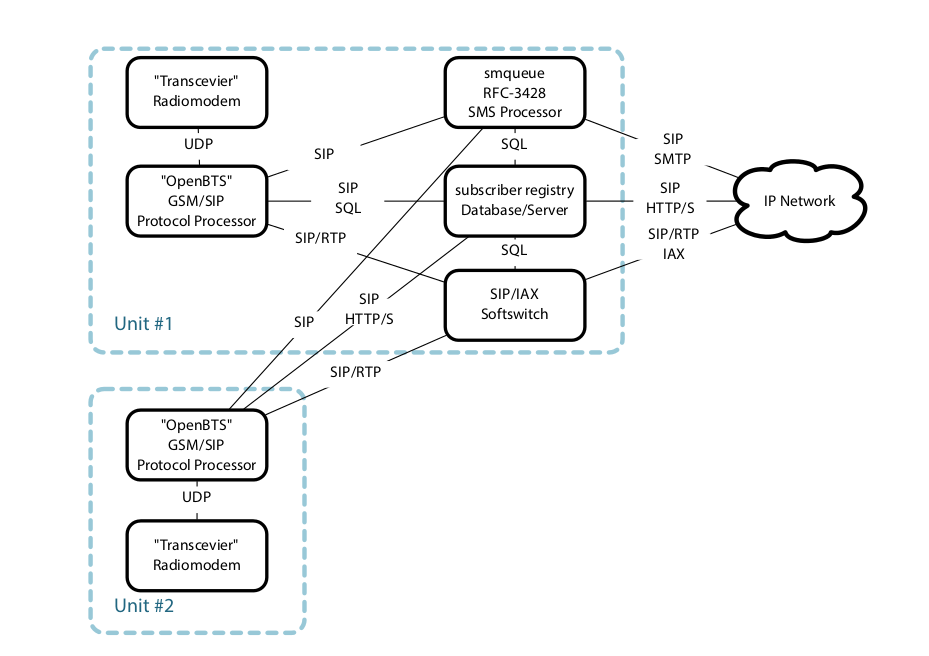
\includegraphics[width=\textwidth]{btsLarge}
  \caption[OpenBTS network with two access points]{Two access points with unit 
  \#1 providing servers for both \protect\cite{openbtsMan}}
  \label{fig:btsLarge}
\end{figure}
